% scratch tex file for trying out stuff for presentation.

% This text is proprietary.
% It's a part of presentation made by myself.
% It may not used commercial.
% The noncommercial use such as private and study is free
% May 2007
% Author: Sascha Frank 
% University Freiburg 
% www.informatik.uni-freiburg.de/~frank/
%
% 
\documentclass{beamer}
\setbeamertemplate{navigation symbols}{}

\usepackage{beamerthemeshadow}
\usepackage{fontawesome}
\usepackage{dashrule}


% added JW:
\usepackage{amsmath}




\begin{document}
\title{SiScLab Project 8}  
\author{Katta, Partmann, Wasmer}
\date{\today} 

% \begin{frame}
% \titlepage
% \end{frame}

\section{Implementation}
\label{sec:implementation}


\newcommand{\aiida}{%
  \begingroup\normalfont
  
\includegraphics[height=1.0\fontcharht\font`\B]{img/aiida_logo.png}%
  \endgroup
}
\newcommand{\aiidalab}{%
  \begingroup\normalfont
  
\includegraphics[height=1.0\fontcharht\font`\B]{img/aiidalab_logo.png}%
  \endgroup
}
\newcommand{\theimage}{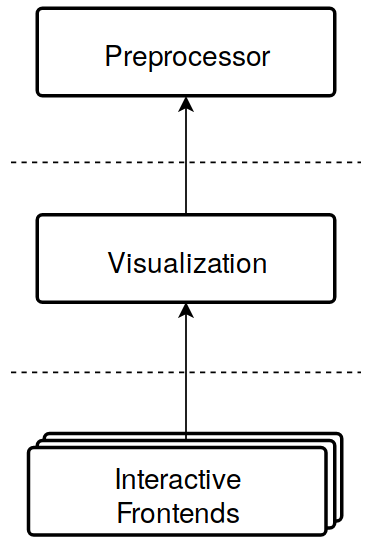
\includegraphics[width=0.8\linewidth]{img/module_design.png}}% Shorthand
\begin{frame}\frametitle{Module Design}
    \begin{columns}
        \begin{column}{.5\textwidth}
            \centerline{\theimage}
        \end{column}
        
        \begin{column}{.5\textwidth}
            \vspace{-2em}
            \begin{itemize}
            \item automated workflows like in \aiida{}
            \item manual data analysis with Python
            \end{itemize}
            \hdashrule{\textwidth}{1pt}{1pt}
            \begin{itemize}
            \item one code for all
            \end{itemize}
            \hdashrule{\textwidth}{1pt}{1pt}
            \begin{itemize}
            \item for Desktop \faDesktop{}
            \item for Web \faGlobe{} like in \aiidalab{}
            \end{itemize}
        \end{column}
    \end{columns}


    
    % TODO \texttt{hdf} preprocessor as self-contained module built for extension
    
    % TODO \texttt{plot} visualization common to all frontends
    
    % TODO \texttt{tk, jupyter} 2 interactive frontends (deployment)
\end{frame}

\subsection{Preprocessor}
\label{sec:preprocessor}

\renewcommand{\theimage}{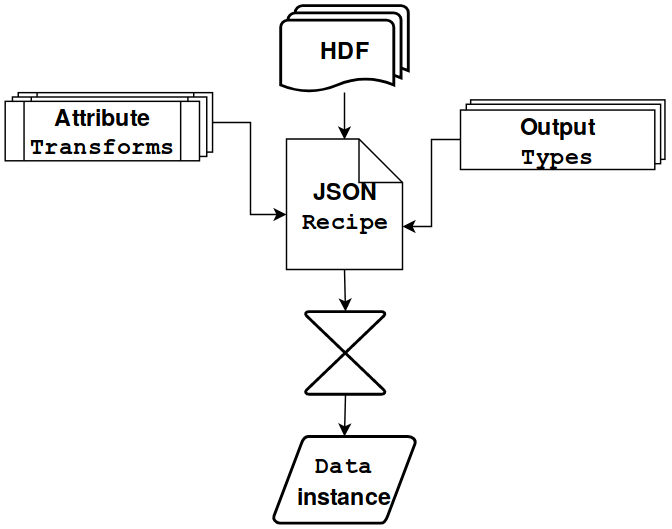
\includegraphics[width=1.2\linewidth]{img/reader_flowchart4.png}}% Shorthand
\begin{frame}\frametitle{Preprocessor Module}
    \begin{columns}
        \begin{column}{.5\textwidth}
            \centerline{\theimage}            
        \end{column}

        \begin{column}{.5\textwidth}
            Input: Hierarchical Data Format (HDF).

            Module uses type introspection to enable features:
            \begin{itemize}
            \item modular output types
            \item dependency resolution
            \end{itemize}

        \end{column}
    \end{columns}
\end{frame}
% Talking Notes:
% - HDF: like a file system with metadata annotation
% - Recipe: build class at runtime (introspection), with transformed attributes (HDF datasets) and
%   application-specific functions, and instantiate object.
% - Dependency resolution: user does not have to take care of order in which
%   arguments are processed (alphabetic ordering)
% - Transforms Dependency example: coordinate transformation
% - Reusability: new recipes may be composed for different workflows with minimal effort
% - Abstract base classes define general and specific Transforms and Output Types
% - Output type example: FleurBands

\subsection{Interactive Visualization}
\label{sec:visualization}

\begin{frame}
    \frametitle{Data Selection}
    \(l\)-like charge density: \(n_{\nu,l}^\mu(\mathbf{k}) = \int_{MT^\mu} |\psi_{\nu,l}^\mu(\mathbf{k,r})| d^3r :\approx L_{skngc}\) 

    The main compute-intensive routine:
    \begin{align*}
      W^{\text{eff}}_{s,\mathbf{k},\nu} = \left( \frac{\sum\limits_{\substack{g \in \text{groups} \\ c \in \text{characters}}} L_{s,\mathbf{k},\nu,g,c} G_g}{\sum\limits_{\substack{g \in \text{all groups} \\ c \in \text{all characters}}} L_{s,\mathbf{k},\nu,g,c} G_g} \right) \left(W_{s,\mathbf{k},\nu}^{\text{unf}}\right)^\alpha
    \end{align*}
\end{frame}
% Slide notes:
% - Reference: Bluegel FLAPW https://www.fz-juelich.de/SharedDocs/Downloads/PGI/PGI-1/DE/SB_NIC_pdf.pdf?__blob=publicationFile
% - indices: nu = band index, mu = muffin tin (i.e. atom, probably corresponds
% to atom group index), l = angular
% quantum number?
% - s = spin, k = k vector, g atom group, G_g atoms_per_group
% - alpha = unfolding weight exponent
% 
% Talking Notes:
% - get_data method

\begin{frame}
    \frametitle{Optimization}
    \begin{itemize}
    \item reshaping \((\mathbf{k},\nu) \rightarrow (\mathbf{k} \cdot \nu\)
    \item weight filter \(t\): \(W^{\text{eff}}_{s,\mathbf{k},\nu} > t\)
    \item TODO ??? \texttt{np.tensor} ???
    \item buffering on selection change
    \end{itemize}
    TODO Result: speedup of about ???factor??? 
\end{frame}

\renewcommand{\theimage}{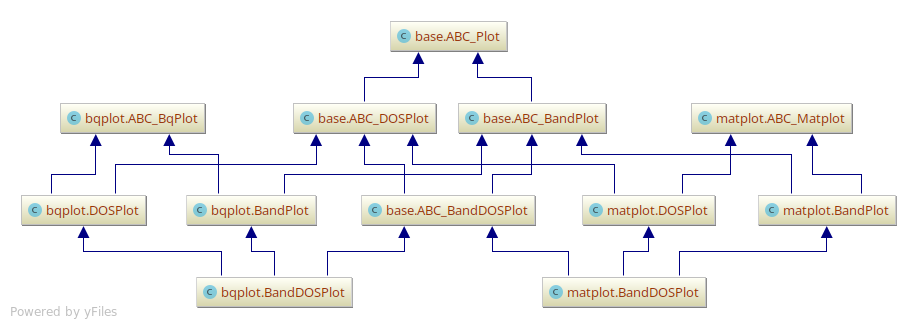
\includegraphics[width=1.1\linewidth]{img/pycharm_uml/matplot.png}}% Shorthand
\begin{frame}\frametitle{Visualization Module}
    \begin{itemize}
    \item Abstract interfaces for different viz. libs and applications
    \item \texttt{InteractiveControlDisplay} as frontend contracts 
    \end{itemize}    
    \centerline{\theimage}
\end{frame}

\subsection{Desktop Frontend}
\label{sec:desktop-frontend}

\begin{frame}\frametitle{Desktop Frontend}
    TODO Praneeth?
\end{frame}

\subsection{Web Frontend}
\label{sec:web-frontend}

\begin{frame}\frametitle{Web Frontend}
    TODO Selection Process from Notes 
\end{frame}

\begin{frame}\frametitle{}
    TODO Selection Process Choices from Notes 
\end{frame}







\end{document}



%%% Local Variables:
%%% mode: latex
%%% TeX-master: t
%%% End:
